\graphicspath{
  {./images/bmps/}{./images/vects/}{./images/}
  {./images/presentation/bmps/}{./images/presentation/vects/}{./images/presentation/}
  {./images/chapter00/bmps/}{./images/chapter00/vects/}{./images/chapter00/}
  {./images/chapter03/bmps/}{./images/chapter03/vects/}{./images/chapter03/}
}

\subsection{Evaluation of Stereo 3D Reconstruction Algorithms}
\begin{frame}{Introduction}
  \begin{itemize}
    \item We want to know the best performance algorithms available for environmental mapping.
    \item Very few datasets $\rightarrow$ Most of them in controlled conditions
    \item Three different and well-known evaluation strategies
    \item Three different dense reconstruction algorithm implementations
    \item Work in collaboration with VisLab.
  \end{itemize}
  \begin{center}
    
\includegraphics[height=0.4\textheight]{vislab_logo}
  \end{center}
  
  \note {
  \begin{itemize}
   \item Critical tasks in the development of driving assistance systems and stereo vision has been widely used to accomplish it
   \item that allow assessing the performance of a specific method in a real world application
   \item conditions... which are not able to capture the variety of the real world
   \item These strategies represent a trade-off btween cost, set up time and accuracy
  \end{itemize}
  }
\end{frame}

\begin{frame}[plain]{Experimental setup}
  \framesubtitle{Dense LIDAR-based ground truth}
  \begin{overlayarea}{\textwidth}{\textheight}
    \begin{itemize}
      \item KITTI dataset from the Karlsruhe Institute of Technology.
      \item Only non-occluded computed pixels have been considered
      \item Average errors have been computed considering only the values below the endpoint error.
      \item Statistics for each frame are being considered, not just their average over an entire sequence.
    \end{itemize}
    
  \end{overlayarea}
  \begin{overlayarea}{\textwidth}{\textheight}
    \only<1> {
      \vspace{-3.5cm}
      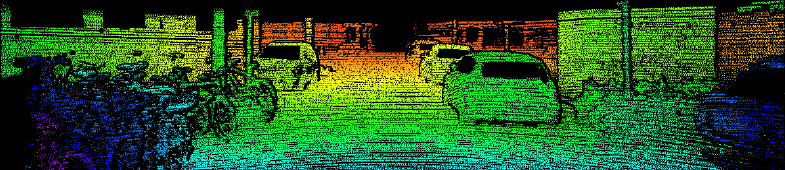
\includegraphics[width=\textwidth]{lidarGT}
    }
    \only<2> {
      \vspace{-4.25cm}
      \begin{center}
	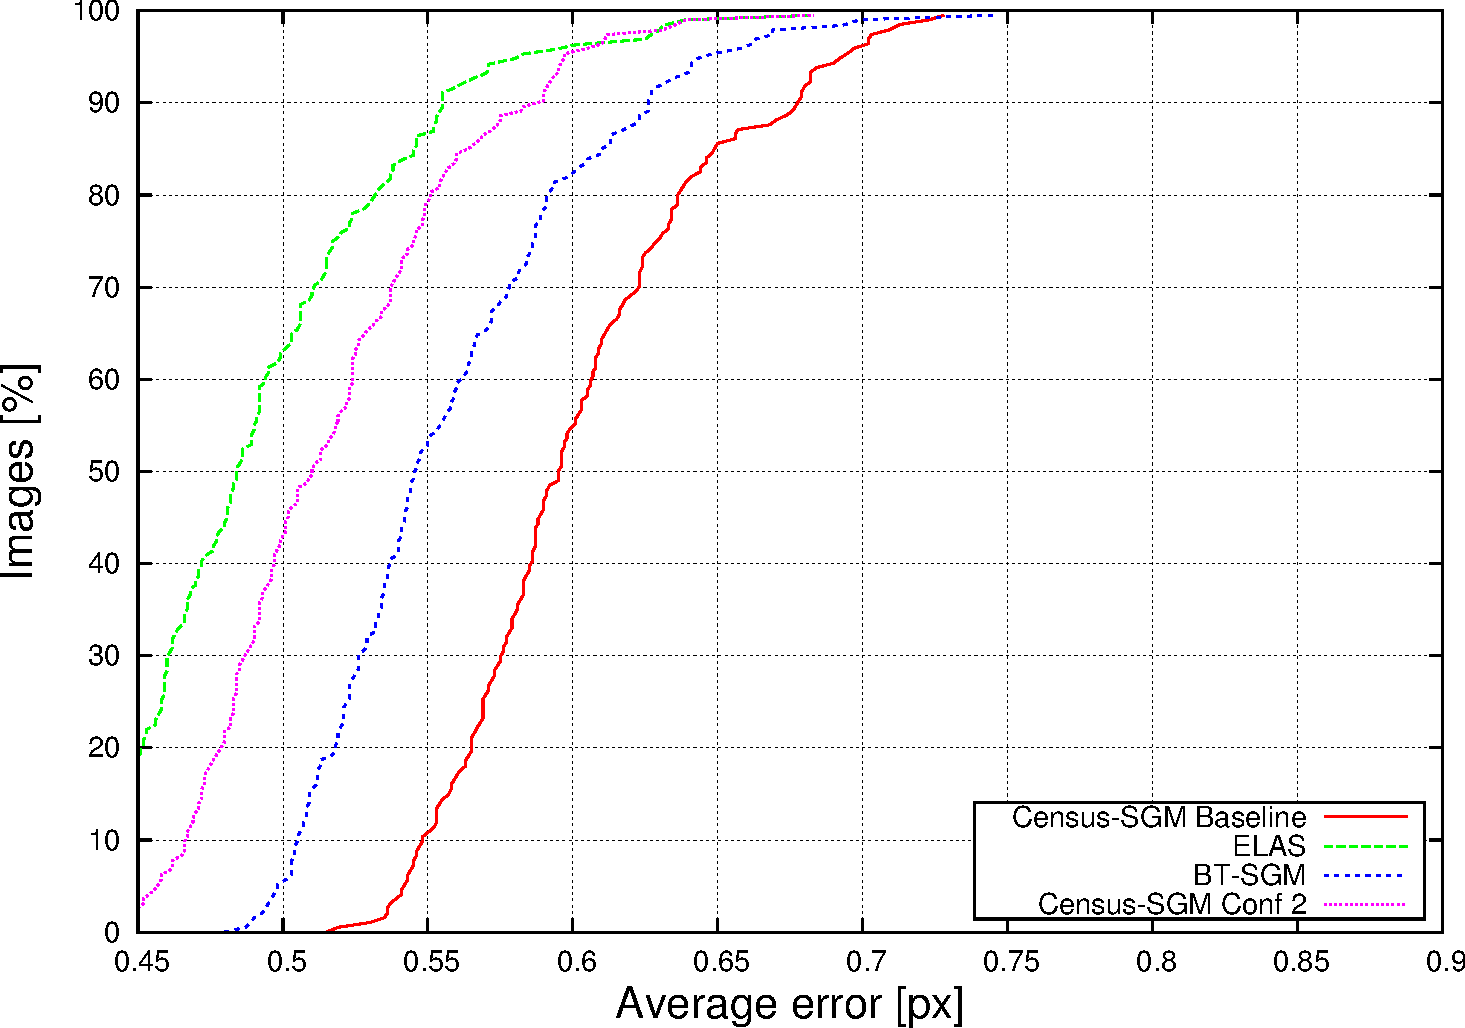
\includegraphics[height=0.6\textheight]{algo_avg_ee2}
      \end{center}
    }
  \end{overlayarea}

  \note {
  \begin{itemize}
    \item Ground truth for a given frame is obtained by registering 5 consecutive frames before and after the one selected and accumulating the resulting point clouds.
    \begin{itemize}
      \item Ambiguous regions such windows and fences are manually removed
      \item The corresponding disparity map is computed using calibration information
    \end{itemize}
    \item The original benchmark also uses linear interpolation of missing values, making sparse and semi-dense methods comparable to dense ones -> This is not fair and hardly optimal // Worsened error metrics for non-dense algorithms.
    \item ... And not all the values
    \item To better understand the collected data, it will be plotted in a graph with the independent variable (x-axis) representing the measured value, and the dependent one (y-axis) the percentage of frames falling below it. Better-performing algorithms are those with a lower x value for a given frame percentage (e.g. y = 90%).
 \end{itemize}
 }
\end{frame}

\begin{frame}{Experimental setup}
  \framesubtitle{False correspondences estimation}
  \begin{itemize}
    \item A safety distance of about 1\,s is usually kept from a leading vehicle.
    \item A speed-dependent free volume is present in front of the ego-vehicle. \\
  \end{itemize}
  \vspace{-0.5cm}
  \begin{center}
    \begin{figure}[t]
	  \centering
	  \begin{subfigure}[t]{0.5\textwidth}
	      \includemovie[autoplay, repeat, controls]{\linewidth}{0.5\textheight}{/home/nestor/Seafile/Videos/Tesis/cp03/FC.avi}
	  \end{subfigure}% 
	  ~
	  \begin{subfigure}[t]{0.5\textwidth}
	      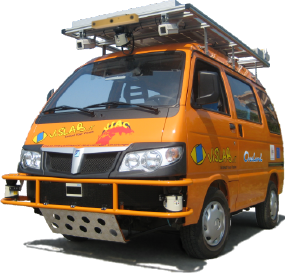
\includegraphics[height=0.5\textheight]{viac_van}
	  \end{subfigure}%       
    \end{figure}
  \end{center}

  \note {
    \begin{itemize}
     \item Any reconstructed point falling within said area must be considered as an erroneous estimate.
     \item We reject false negatives using the LIDAR information.
     \item Face correspondences percentage is the ratio of points inside the object-free volume respect to the total number of 3D points.
    \end{itemize}
  }
\end{frame}

\begin{frame}{Experimental setup}
  \framesubtitle{Normalized Cross Correlation (NCC)}

  \begin{center}
    \begin{figure}[t]
	  \centering
	  \begin{subfigure}[t]{0.5\textwidth}
	    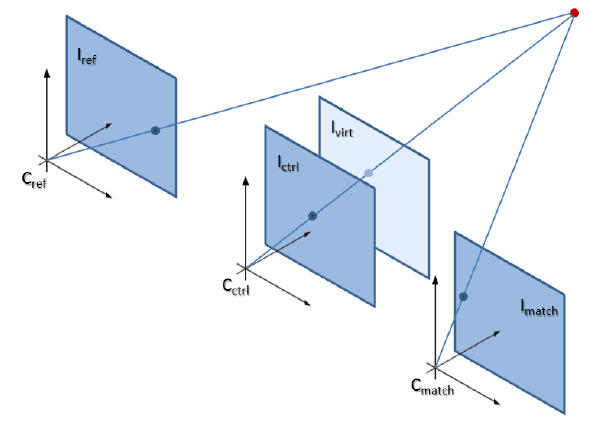
\includegraphics[width=\textwidth]{trinocular_setup}
	  \end{subfigure}% 
	  ~
	  \begin{subfigure}[t]{0.5\textwidth}
	    \includemovie[autoplay, repeat, controls]{\linewidth}{0.5\textheight}{/home/nestor/Seafile/Videos/Tesis/cp03/ncc.avi}	      
	  \end{subfigure}%       
    \end{figure}
  \end{center}

  \note {
    \begin{itemize}
     \item LIDAR-based GT takes time to be produced and FC is an indirect measurement.
     \item The use of a third camera allows to directly compare a reconstructed view with the actual images w/o manual intervention.

     \item NCC is calculated as described by Morales et al.

     \item It is suggested a configuration of 20 cm btween ref and match, and the ctrol camera is at 50 cm from ref camera
     \item In our conf, it is 24 and 12, respectively, as we use a precalibrated trinocular camera.
    \end{itemize}
  }
\end{frame}
